\chapter{Unit Tests} \label{sec:results}


\section{10 Unit Tests}

\autoref{tab:tests} zeigt die geforderten Tests. 

\newcounter{rowcounter}
\newcommand\rownumber{\stepcounter{rowcounter}\arabic{rowcounter}}

\newcolumntype{b}{X}
\newcolumntype{s}{>{\hsize=.5\hsize}X}

\begin{table}[H]
	\centering
	\begin{tabularx}{\textwidth}{rs|b}
		& \textbf{Unit Test} & \textbf{Beschreibung} \\
		\midrule
		\rownumber & RollIntegerTest \#fromNumberCappedTest & 
		Testet statische \textit{fromNumberCapped}-Funktion der \textit{RollInteger}-Klasse, ob das richtige, ggf. beschränkte, Ergebnis 
		erzeugt wird, bzw. illegale Eingaben abgewiesen werden. \\ 
		\rownumber & Roll\#raiseRollByTest &
		Testet \textit{raiseRollBy}-Methode der \textit{Roll}-Klasse, ob die Erhöhung den Domänenregeln entsprechend durchgeführt wird. \\
		\rownumber & RollHandlerTest \#encounter &
		Testet encounter-Methode des RollHandler auf verschiedenen legalen Input von gemocktem Bonusschaden, Tieren und Würfelwürfen. \\
		\rownumber & RollHandlerTest \#endeavor & Testet endeavor-Methode des RollHandler mit RescueMock mit verschiedenen Ergebnissen. \\
		\rownumber & CollectionStringerTest \#collectionToStringTest &
		Testet \textit{collectionToString}-Methode der \textit{CollectionStringer}-Klasse,
		ob die String-Konvertierung insb. mit den Zeilenumbrüchen ordentlich funktioniert. \\
		\rownumber & DiceParserTest \#parseTest &
		Testet \textit{parse}-Methode der \textit{DiceParser}-Klasse,
		ob die verschiedenen Würfeltypen und Augenzahlen, sowie die Random-Roll-Funktion für die jeweiligen Würfel korrekt parsen. \\
		\rownumber & NonNegativeIntegerTest \#addTest & 
		Testet add-Methode von NonNegativeInteger gründlich, ob richtiges Ergebnis erzeugt wird bzw. illegale Eingaben abgewiesen werden \\ 
		\rownumber & NonNegativeIntegerTest \#newNonNegativeIntegerTest & 
		Testet Konstruktor von NonNegativeInteger ungründlich, ob Eingabe zugelassen wird. \\ 
		\rownumber & ResourceStashTest \#devastateTest &
		Testet \textit{devastate}-Methode der \textit{ResourceStash}-Klasse,
		ob die Ressourcen bis auf genau die obersten $n$ gelöscht werden. \\
		\rownumber & ResourceStashTest \#hasResourcesTest &
		Testet \textit{hasResources}-Methode der \textit{ResourceStash}-Klasse,
		ob verschiedene \textit{ResourceRequirements} immer korrekt behandelt werden. \\

	\end{tabularx}
	\caption{Zehn Unit Tests mit Namen (ausgehend von \textit{de.dhbw.karlsruhe.ase}) und Beschreibung. (Packages ausgelassen aus Platzgründen).}
	\label{tab:tests}
\end{table}


\section{ATRIP: Automatic}

\textit{Automatic} verlangt, dass mit minimalem Aufwand die Ausführung der Unit Tests angestoßen werden kann. Hierfür 
wird das Unit-Testing-Framework \textit{JUnit} verwendet, wonach Methoden erstellt werden können, die mit \textit{@Test} annotiert sind, 
wodurch sie durch JUnit ausgeführt werden, wenn über die IDE oder Maven ein entsprechender Befehl erfolgt. Zur Unterstützung 
der automatisierten Ausführung sind die Unit Tests so geschrieben, dass sie \textit{Repeatable} und \textit{Independent} sind, 
damit es keine Probleme bei der (wiederholten) automatischen Ausführung der Tests in beliebiger Reihenfolge gibt. Außerdem haben die 
Tests keine externen Abhängigkeiten - auch nicht zu diversen Dateien mit Testinhalten oder Ähnliches. Nach Durchführen der Tests 
gibt JUnit eine Übersicht über die erfolgreichen und ggf. fehlgeschlagenen Tests. Es sind keine Nutzereingaben notwendig. 
Es muss nichts weiter konfiguriert 
werden, um die Tests durchzuführen. Der Konsolenbefehl \texttt{mvn test} genügt direkt nach dem Klonen des Repositorys. 

\section{ATRIP: Thorough}

\subsubsection{Positiv-Beispiel}

\autoref{code:thorough-positive} zeigt das Positiv-Beispiel zu \textit{thorough} Test-Code. Hier wird 
die \textit{add}-Methode der \textit{NonNegativeInteger}-Klasse getestet, die auf einen bestehenden 
NonNegativeInteger einen Java-Integer-Primitive addiert, der sowohl negativ als auch positiv sein kann (solange 
die Summe/Differenz nicht-negativ ist) und das Ergebnis als neuen NonNegativeInteger zurückgibt. Ist das 
Resultat negativ, soll eine \textit{IllegalArgumentException} geworfen werden. \\
Der Test ist thorough, weil durch den \textit{ParameterizedTest} und die dazugehörige \textit{MethodSource} \textit{add}
Stichproben getestet werden, die die Verteilung der möglichen Eingaben \textit{gründlich} abdecken sollten, 
da positive Standardfälle, Edge-Cases und pathologische Eingaben getestet werden.    

\lstinputlisting[
	label=code:thorough-positive,    % Label; genutzt für Referenzen auf dieses Code-Beispiel
	caption=\underline{\textit{Thorough}} Test-Code zur \textit{add}-Methode der \textit{NonNegativeInteger}-Klasse.,
	captionpos=b,               % Position, an der die Caption angezeigt wird t(op) oder b(ottom)
	style=EigenerJavaStyle,   % Eigener Style der vor dem Dokument festgelegt wurde
	firstline=13,                % Zeilennummer im Dokument welche als erste angezeigt wird
	lastline=43                 % Letzte Zeile welche ins LaTeX Dokument übernommen wird
]{Quellcode/thorough.java}

\subsubsection{Negativ-Beispiel}

\autoref{code:thorough-negative} zeigt das Negativ-Beispiel zu \textit{thorough} Test-Code. Hier wird 
der Konstruktor der \textit{NonNegativeInteger}-Klasse getestet, der über eine \textit{IllegalArgumentException} 
sicherstellen muss, dass der übergebene Java-Integer-Primitive nicht negativ, also $\geq 0$ ist. \\
Der Test ist \textit{nicht} thorough, weil durch den Test nur ein einziger positiver Fall ($5 \geq 0$) getestet 
wird, keine Edge-Cases (Eingabe = \textit{Integer.MAX\_INT}, Eingabe = $0$) oder pathologischen Eingaben 
(z.B. Eingabe = $-3$) getestet werden. Die Hauptfunktionalität - also das Ablehnen von negativen Eingaben zum 
Einhalten des Vertrags - wird so nicht ein mal getestet und damit eigentlich nur triviales Konstruktorverhalten.

\lstinputlisting[
	label=code:thorough-negative,    % Label; genutzt für Referenzen auf dieses Code-Beispiel
	caption=\underline{Nicht} \textit{thorough} Test-Code zum Konstruktor der \textit{NonNegativeInteger}-Klasse.,
	captionpos=b,               % Position, an der die Caption angezeigt wird t(op) oder b(ottom)
	style=EigenerJavaStyle,   % Eigener Style der vor dem Dokument festgelegt wurde
	firstline=45,                % Zeilennummer im Dokument welche als erste angezeigt wird
	lastline=50                 % Letzte Zeile welche ins LaTeX Dokument übernommen wird
]{Quellcode/thorough.java}

\section{ATRIP: Professional}

\subsubsection{Positiv-Beispiel}

\autoref{code:pro-positive} zeigt das Positiv-Beispiel zu \textit{professional} Test-Code. Hier wird die 
\textit{raiseRollBy}-Methode der \textit{Roll}-Klasse getestet, die einen bestehenden \textit{Roll} 
um einen \textit{NonNegativeInteger} erhöhen soll, aber nur bis zu dem maximalen legalen Wert des bestehenden Rolls, 
der abhängig von dessen \textit{DiceType} ist, und das Resultat als neuen Roll zurückgeben soll. \\
Der Test ist professionell da keinerlei Code-Duplication vorliegt und das SRP eingehalten ist, 
da der Test als \textit{ParameterizedTest} all die Test-Cases, die durch die \textit{MethodSource} gegeben sind, ausführt.
Durch den ParameterizedTest ist auch leicht zu erkennen, welche Test-Cases erfolgreich waren und welche nicht. 
Die Variablen- und Methodennamen sind leicht verständlich und der Code ist gut lesbar. 
Es bestehen auch keine sonstigen Code-Smells. Zudem testet der Test eine relevante und nicht-triviale Methode, 
die wichtig für das Einhalten der Domänenregeln ist und deswegen korrekt sein muss, ansonsten würden Bugs 
verteilt in der Codebase auftreten.  

\lstinputlisting[
	label=code:pro-positive,    % Label; genutzt für Referenzen auf dieses Code-Beispiel
	caption=\underline{Professioneller} Test-Code zur \textit{raiseRollBy}-Methode der \textit{Roll}-Klasse.,
	captionpos=b,               % Position, an der die Caption angezeigt wird t(op) oder b(ottom)
	style=EigenerJavaStyle,   % Eigener Style der vor dem Dokument festgelegt wurde
	firstline=13,                % Zeilennummer im Dokument welche als erste angezeigt wird
	lastline=61                 % Letzte Zeile welche ins LaTeX Dokument übernommen wird
]{Quellcode/professional.java}

\subsubsection{Negativ-Beispiel}

\autoref{code:pro-negative} zeigt das Negativ-Beispiel zu \textit{professional} Test-Code. Hier wird die 
statische \textit{fromNumberCapped}-Funktion der \textit{RollInteger}-Klasse getestet, die aus einem Java-Integer-Primitive und 
einem \textit{DiceType} einen neuen RollInteger erstellen soll, dessen Wert dem Primitive entspricht, aber maximal 
dem Maximalwert des übergebenen DiceType. Zahlen $< 1$ sollen durch eine \textit{IllegalArgumentException} abgefangen werden. \\
Der Test ist unprofessionell aus folgenden Gründen:
\begin{enumerate}
	\item Es besteht extrem viel Code-Duplication, da der Test wohl durch Copy-Paste erzeugt wurde. 
	Dies sollte durch eine Method-Extraction behoben werden. 
	\item Alle Test-Cases stehen in der einen Test-Methode ($\rightarrow$ SRP verletzt), wodurch es schwieriger wird bei 
	teilweise fehlschlagenden Assertions zu erkennen, wo der Fehler liegt. Die Test-Cases sollten in eigene Tests ausgelagert werden, 
	sodass das SRP gewahrt wird. Zusammen mit dem vorherigen Punkt sollte also ein \textit{ParameterizedTest} mit \textit{MethodSource}
	für die Test-Cases erstellt werden.
	\item Es werden die temporären Variablen \textit{inputInteger} und \textit{inputDiceType} nicht konsequent angewandt, 
	sondern trotzdem noch magische Konstanten (s. z.B. Zeile 15, wo eine $2$ steht, statt \textit{inputInteger}). 
	\item Bei den Tests, bei denen der \textit{inputInteger} das Maximum des Würfeltyps überschreitet (z.B. Block Zeile 17 ff.), 
	sollte keine magische Konstante (im Beispiel $6$ für \textit{DiceType.SIX\_SIDED}) als erwarteter Wert verwendet werden,
	sondern \textit{inputDiceType.integerRepresentation}, welche das Maximum darstellt.
	\item In Zeile 35 steht ein Multiline-Kommentar mitten im Code, um eine magische Konstante zu erklären. Um diesen Code-Smell aufzuheben,
	sollte die Konstante \textit{Integer.MIN\_VALUE} eingefügt werden.
\end{enumerate}

\lstinputlisting[
	label=code:pro-negative,    % Label; genutzt für Referenzen auf dieses Code-Beispiel
	caption=\underline{\textbf{Un}professioneller} Test-Code zur statischen \textit{fromNumberCapped}-Funktion der \textit{RollInteger}-Klasse.,
	captionpos=b,               % Position, an der die Caption angezeigt wird t(op) oder b(ottom)
	style=EigenerJavaStyle,   % Eigener Style der vor dem Dokument festgelegt wurde
	firstline=8,                % Zeilennummer im Dokument welche als erste angezeigt wird
	lastline=46                 % Letzte Zeile welche ins LaTeX Dokument übernommen wird
]{Quellcode/unprofessional.java}

\section{Code Coverage}

\begin{table}[H]
	\centering
	\begin{tabular}{l|l|l}
	Line & Method & Class \\
	\midrule
	91\% (611/671) & 95\% (237/249) & 100\% (67/67) 
	\end{tabular}
	\caption{Code-Coverage der Tests relativ und absolut nach Statement-, Method- und Class-Coverage.}
	\label{tab:coverage}
\end{table}

\autoref{tab:coverage} zeigt die Code-Coverage aller Tests im Projekt nach Statement-, Method- und Class-Coverage sowohl als relativer (prozentualer) Wert, 
als auch als absoluter Wert. Der Wert von 91\% Statement-Coverage wird als gut für das konkrete Projekt angesehen. Insbesondere, wenn beachtet wird, 
welche Zeilen nicht abgedeckt sind: zumeist das Werfen von Runtime-Exceptions oder das Behandeln von Exceptions im Plugin-Code in Form von 
Fehlerausgaben an den Nutzer. Es gibt zwar kein allgemein anerkannten Wert für eine \enquote{gute} Code-Coverage, aber für ein brettspielartiges 
Kartenspiel ist dies ein ausreichender Wert, da keine größeren Bugs vorhanden sein sollten und das Spiel im Großen und Ganzen gut funktionieren sollte,
abgesehen von möglicherweise ein paar wenigen kleineren Bugs. Insbesondere die Blackbox-Integration-Tests sichern einen normalen Spielverlauf zu. 
Da es sich außerdem um kein Online-Spiel handelt und es keine Leaderboards gibt, muss das Spiel auch nicht zu sehr auf diverse kleinere Exploits 
oder Glitches getestet werden. Für andere, sicherheitskritische Software wäre eine Code-Coverage von 91\% sicher unzureichend, aber für dieses 
Anwendung ist es ausreichend.       


\section{Fakes und Mocks}

\subsubsection{CampMock}

\autoref{fig:CampMock} zeigt das UML-Diagramm eines Mocks zum Testen der \textit{encounter}-Methode des \textit{RollHandler}. 
Der \textit{CampMock} ist realisiert als Subklasse der zu mockenden Oberklasse \textit{Camp}, wobei CampMock die relevanten 
zu mockenden Methoden überschreibt. Konkret ist das hier lediglich die \textit{getBonusDamage}-Methode, die im Mock das private
Attribut \textit{bonusDamage} zurückgibt, welches durch den Konstruktor gesetzt wird. \\ 
Grund für den Mock ist, dass in der encounter-Methode auf die getBonusDamage-Methode von Camp zurückgegriffen wird, um zu bestimmen,
ob ein Spieler gegen ein Tier gewinnt oder nicht. Das Setup, um ein Camp zu erzeugen, wobei die getBonusDamage-Methode tatsächlich 
einen gewünschten Wert zurückgibt wäre aber ohne Mock unverhältnismäßig schwierig, da zunächst genügend Ressourcen in das Camp 
eingefüllt werden müssten, dass es reicht ein \textit{Tool} zu bauen, wovon der bonusDamage genommen wird. Außerdem könnten dann 
nur bereits über Tools implementierte Werte für getBonusDamage getestet werden und nicht beliebige. Daher wird hier ein Mock benötigt.     

\begin{figure}[H]
	\centering
	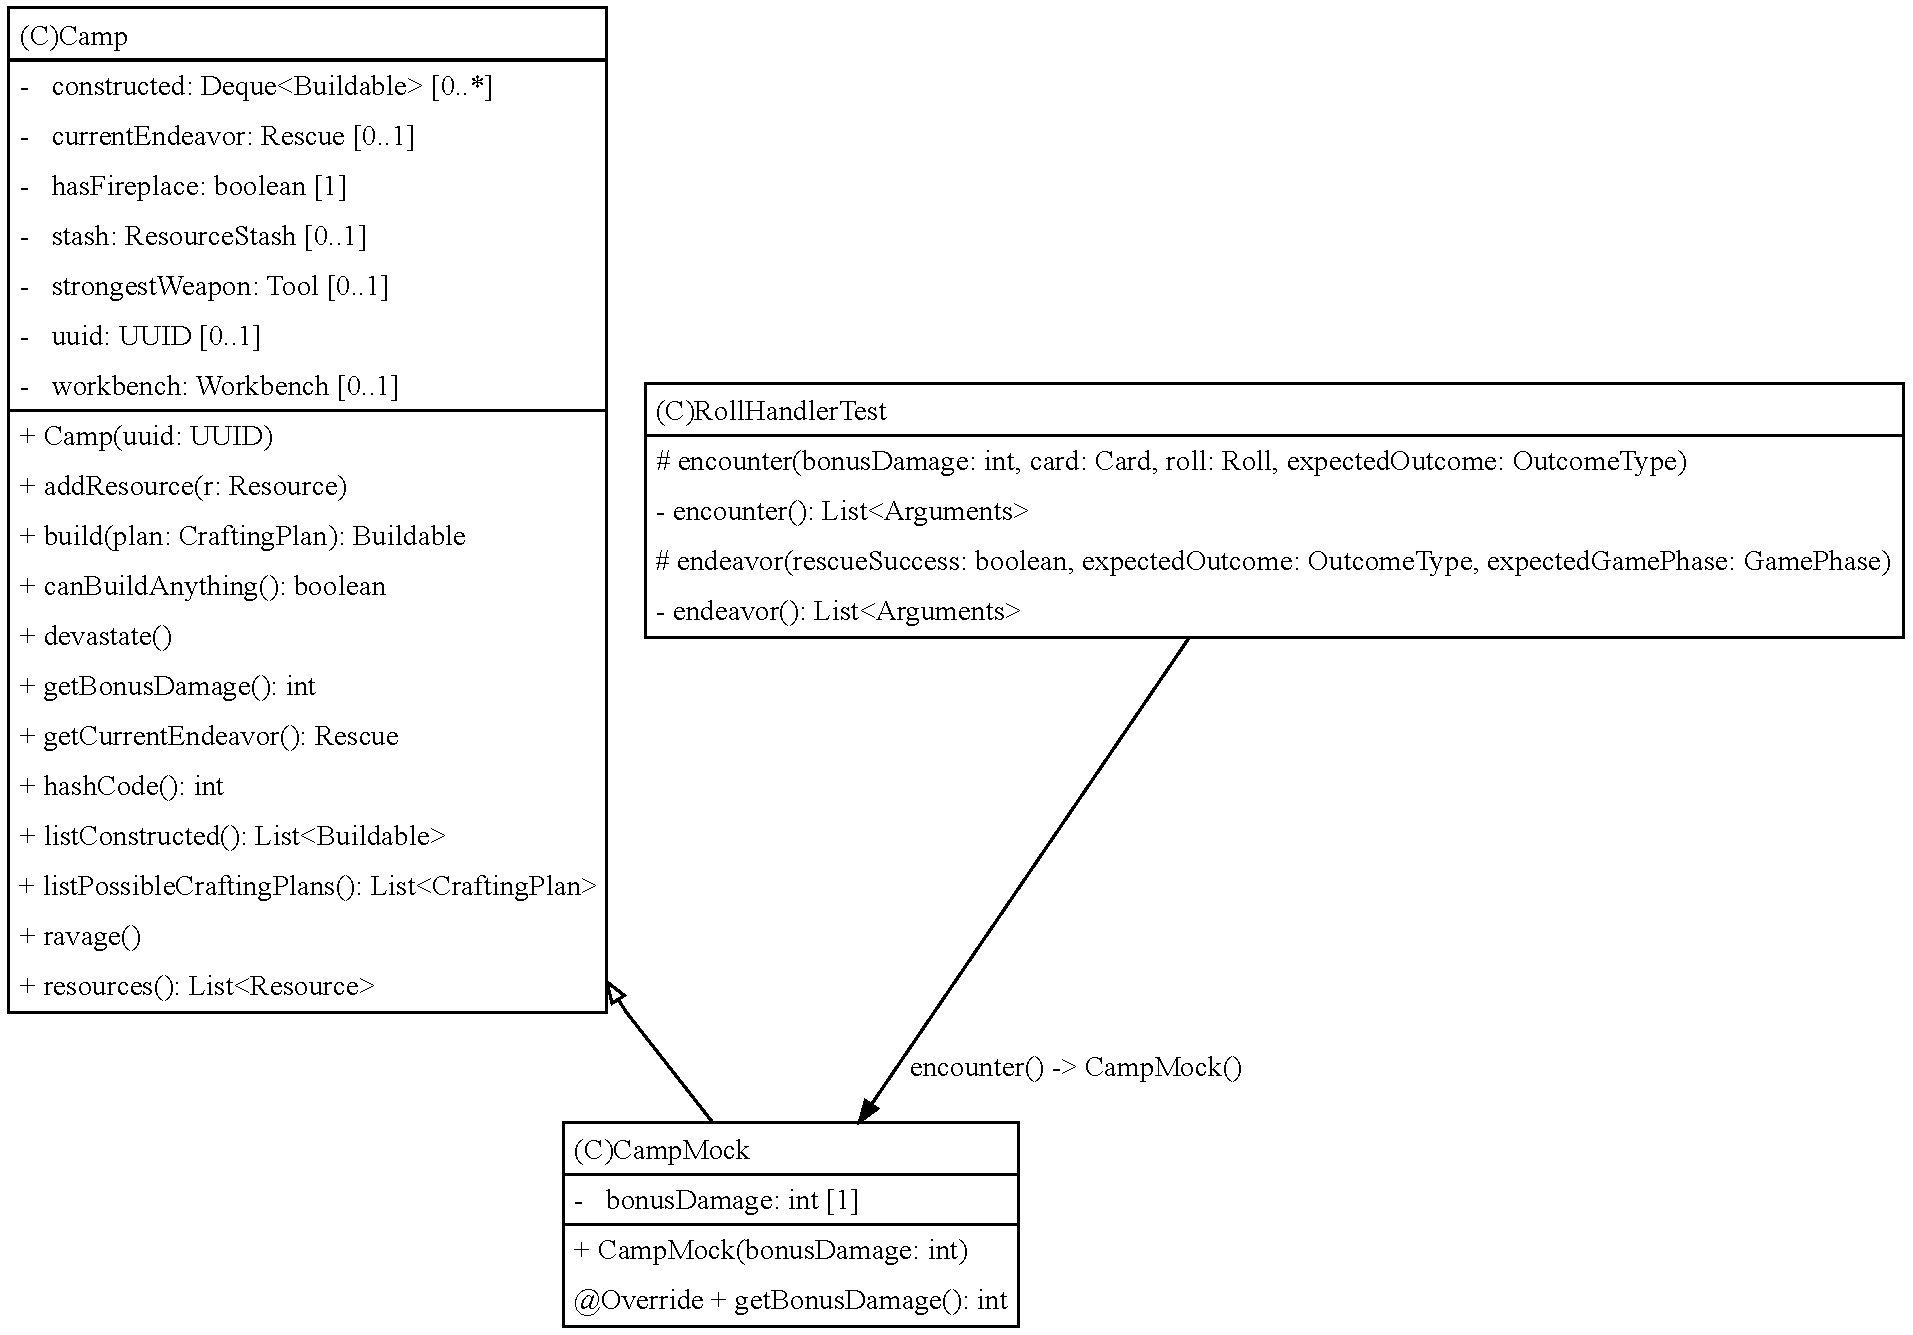
\includegraphics[width=1\textwidth]{Bilder/CampMock_structure.pdf} 
	\caption{UML-Diagramm des \textit{CampMock}, der zur Testung der \textit{encounter}-Methode des \textit{RollHandler} benötigt wird.} 
	\label{fig:CampMock}
\end{figure} 

\subsubsection{RescueMock}

\autoref{fig:RescueMock} zeigt das UML-Diagramm eines Mocks zum Testen der \textit{endeavor}-Methode des \textit{RollHandler}. 
Der \textit{RescueMock} ist realisiert als Implementation des zu mockenden Interfaces \textit{Rescue}, wobei RescueMock die endeavor-Methode 
so überschreibt, dass ein Boolean-Wert zurückgegeben wird, der zuvor über den Konstruktor von RescueMock injiziert wurde. \\ 
Grund für den Mock ist, dass in der endeavor-Methode auf die getCurrentEndeavor-Methode von Camp zurückgegriffen wird, um auf dem 
zurückgegebenen Interface die endeavor-Methode aufzurufen, um zu überprüfen, ob der Spieler von der Insel entfliehen kann. 
Hierfür wird also in Camp der RescueMock injiziert, sodass getCurrentEndeavor den Mock zurückgibt. 
Das Setup, um ein Camp zu erzeugen, welches eine Rescue hält, die einen gewünschten Wert zurückgibt wäre aber ohne Mock unverhältnismäßig schwierig,
da zunächst genügend Ressourcen in das Camp eingefüllt werden müssten, dass es reicht eine \textit{Rescue} zu bauen, 
deren endeavor-Methode den gewünschten Wert zurück gibt. Außerdem könnten dann 
nur bereits über Rescues implementierte Verhalten für Rescue\#endeavor getestet werden und nicht beliebige. Zusätzlich würde 
der Test dann auch die Rescue\#endeavor-Methode der konkreten Rescues testen und nicht nur isoliert die RollHandler\#endeavor-Methode.
Daher wird hier ein Mock benötigt.     

\begin{figure}[H]
	\centering
	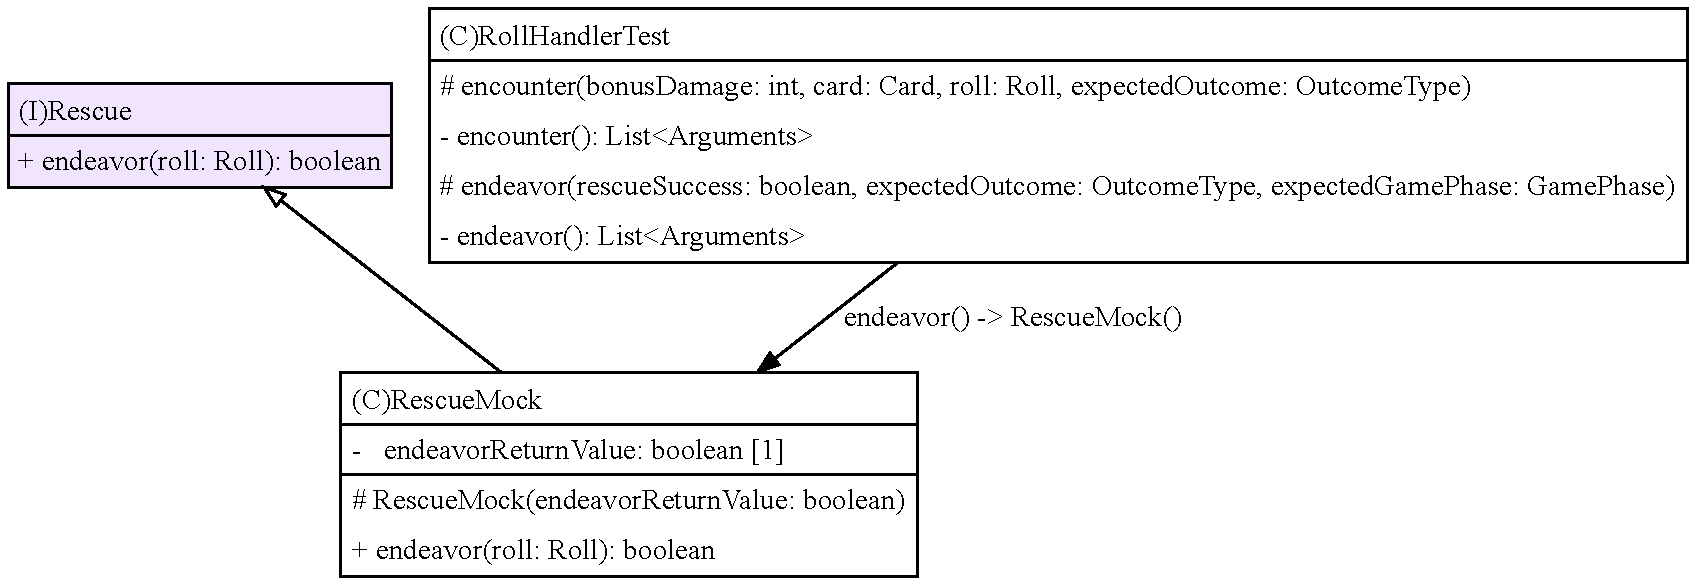
\includegraphics[width=1\textwidth]{Bilder/RescueMock_structure.pdf} 
	\caption{UML-Diagramm des \textit{RescueMock}, der zur Testung der \textit{endeavor}-Methode des \textit{RollHandler} benötigt wird.}
	\label{fig:RescueMock}
\end{figure} 